\documentclass[10pt]{beamer}

\usetheme[progressbar=frametitle]{metropolis}
\usepackage{appendixnumberbeamer}

\usepackage{booktabs}
\usepackage[scale=2]{ccicons}

\usepackage{pgfplots}
\usepgfplotslibrary{dateplot}

\usepackage{graphicx}

\usepackage{xspace}
\newcommand{\themename}{\textbf{\textsc{metropolis}}\xspace}

\newcommand*{\github}{
\includegraphics[width=1.7em]{github}}

\title{Fishy Cyber Attack Detection in \newline Industrial Control Systems}
\subtitle{Zone-Based PCA and\newline A new approach based on LSTM}
% \date{\today}
\date{}
\author{Manikanta Reddy D.}
\institute{IIT Kanpur}
% \titlegraphic{\hfill\includegraphics[height=1.5cm]{logo.pdf}}

\begin{document}

\maketitle

\begin{frame}{Table of contents}
  \setbeamertemplate{section in toc}[sections numbered]
  \tableofcontents[hideallsubsections]
\end{frame}

\section{Introduction}

\begin{frame}[fragile]{Industrial Control Systems}
	
    Industrial Control Systems (ICS) are connected to Internet for information exchange and control transfer.
    
    This potentially exposes the critical system to various side channel attacks.
  
\end{frame}
\begin{frame}[fragile]{The Problem with ICS}
	Security Patches are rarely applied, as they could cause other critical failures.
    
    \begin{alertblock}{Detect and Shutdown}
    	In ICS the norm is to cure rather than to prevent the disease.
        
        \emph{Detect the attack} and \emph{shutdown} the systems to             prevent any damage.
        
        Later fix the problem.
        
        It is important to build a reliable manipulation detection 		         system.
    \end{alertblock}
\end{frame}

\section{Water Plant}

\begin{frame}{Hot Water Plant}
	We'll emulate a simple hot water plant, to test our systems.
    
    The plant consists of hot water circulating between two tanks.
    
    One tank heats and the other lets it cool down.
    
    A pump circulates the water
\end{frame}

\begin{frame}
	\begin{figure}
		\centering
		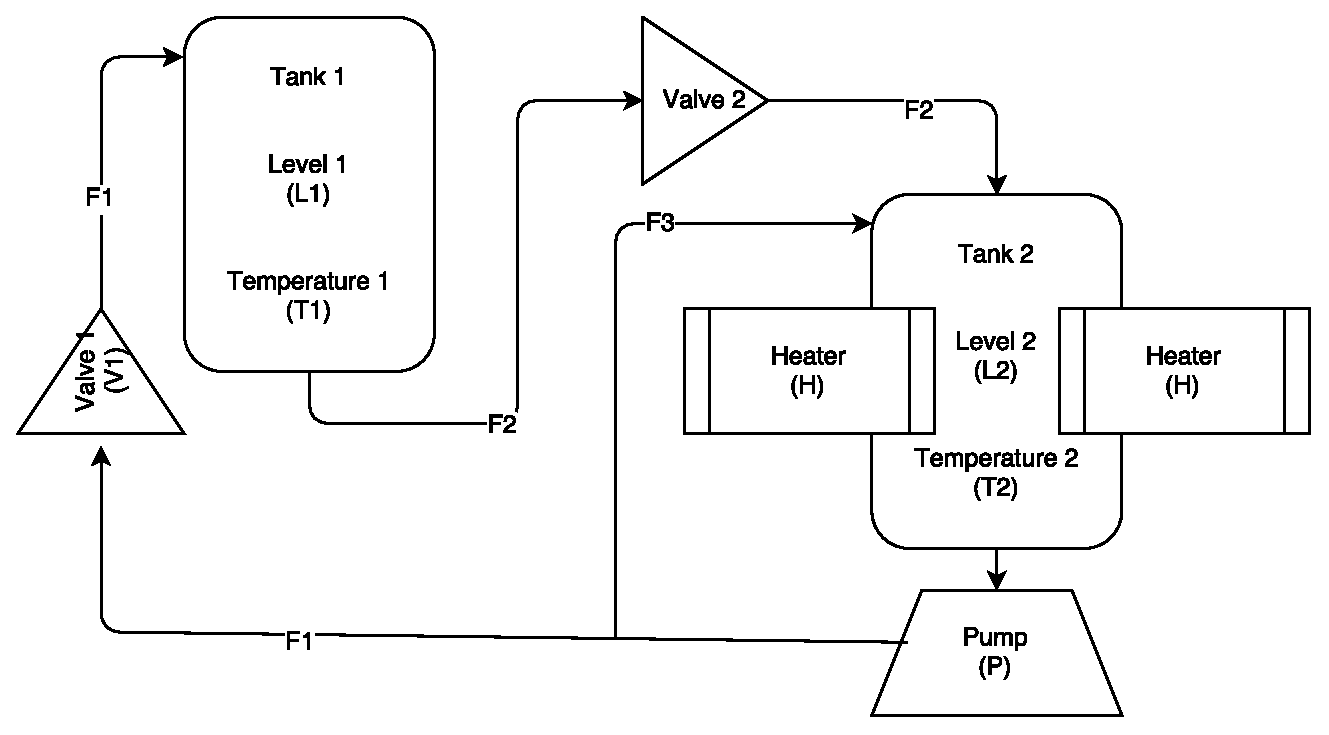
\includegraphics[width=\textwidth]{plant.eps}
		\caption{\label{fig:CN}Hot Water Plant}
	\end{figure}
\end{frame}

\begin{frame}{Attack Detection}
	There are 11 process variables in the system.
    
    Control Variables: V1, V2, P, H
    
    Process Variables: L1, L2, T1, T2, F1, F2, F3
	
    \begin{center}
    	
    \end{center}
	
	In reality there could be many more.
    
    Impossible to monitor all of them concurrently for any manipulation.
\end{frame}

\section{Zone Division\cite{hashimoto2013safety}}

\begin{frame}{An attempt to minimize risk}
	Divide the entire system into zones.
    
    One zone is compromised, try to detect it in other zones.
    
    Allow for cross control and prevent control of variables in the same zone.
    
    A controller in a zone is not allowed to manipulate the variables that change the variables it measures.
\end{frame}

\begin{frame}{Zone Division}
	\begin{figure}
		\centering
		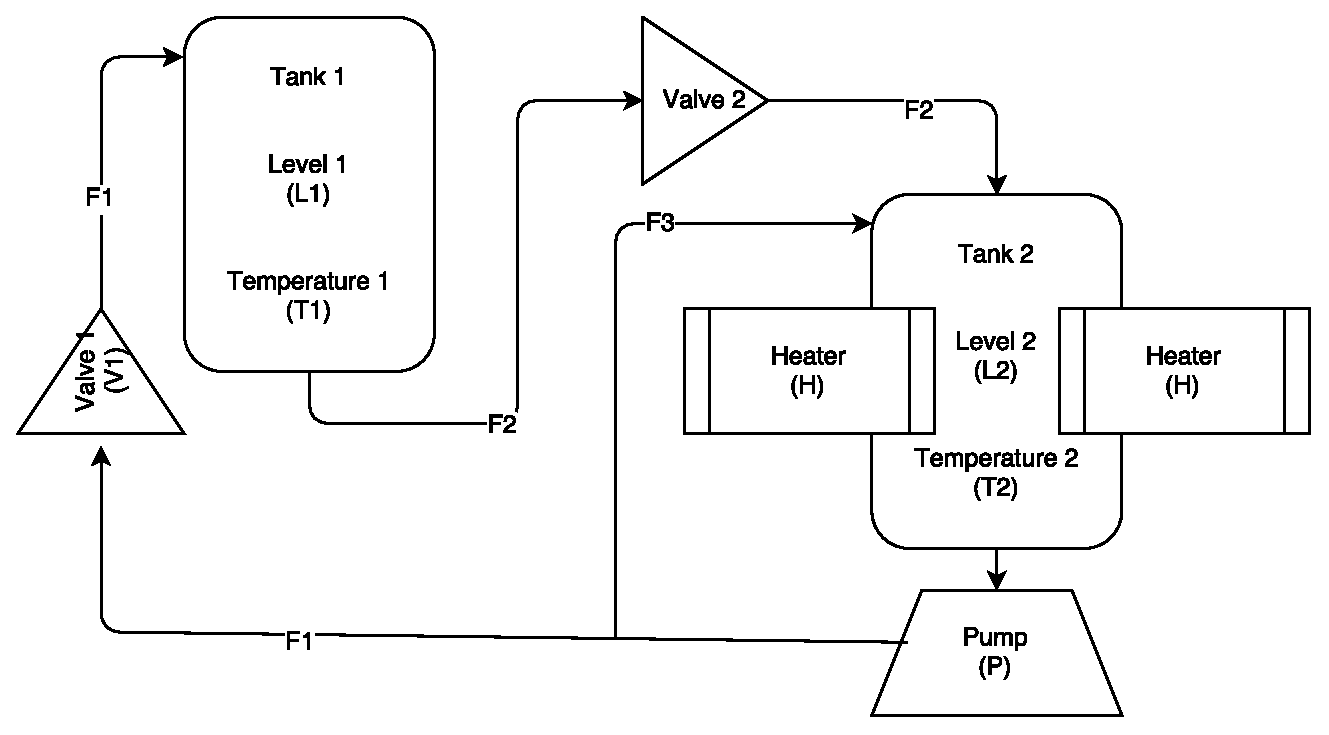
\includegraphics[width=\textwidth]{plant.eps}
	\end{figure}
    Zone1: L1, T1, V2, F2, H
    
    Zone2: L2, T2, V1, F1, F3, P
\end{frame}

\begin{frame}
	\begin{figure}
		\centering
		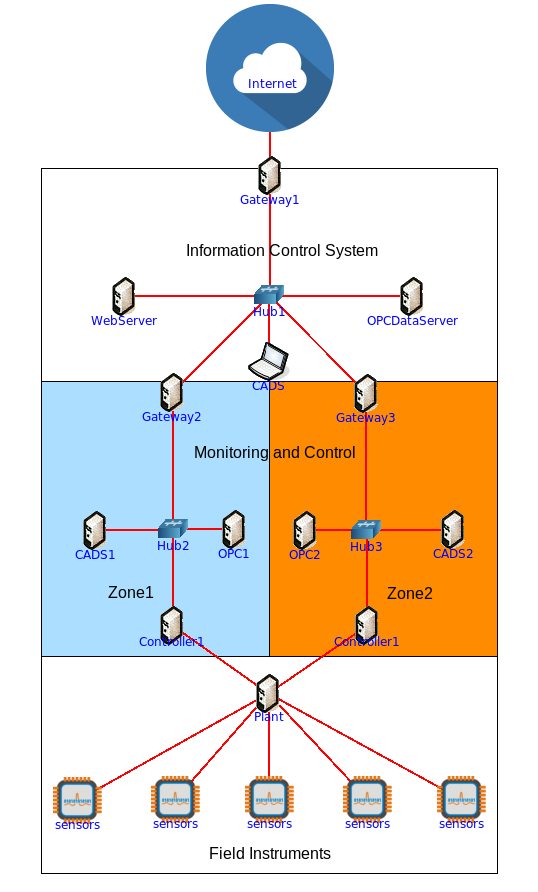
\includegraphics[width=0.5\textwidth]{ControlNetwork.png}
	\end{figure}
\end{frame}


\section{Principal Component Analysis Based Detection\cite{morita2013detection}}

\begin{frame}{The Problem}
	It is very difficult to monitor all process variables concurrently. 
    
    Attacker can also mask the incorrect readings from the compromised zone.
    
    Good Luck with that.
\end{frame}

\begin{frame}{Detect the Change}
	Instead detect only the change. 
    
    Device a method to extract the ones that change the most.
    
    Monitor it and you are done.
    
    This is exactly what PCA based method does.
\end{frame}

\begin{frame}{PCA}
	Prinicipal component analysis reprojects the data into a new space along maximum variance.
    
    Monitor values along these components and any change should be visible. (That too in a magnified fashion).
    
    We have considered 3 PCA components to monitor.
\end{frame}

\begin{frame}
  \begin{figure}
    \centering
    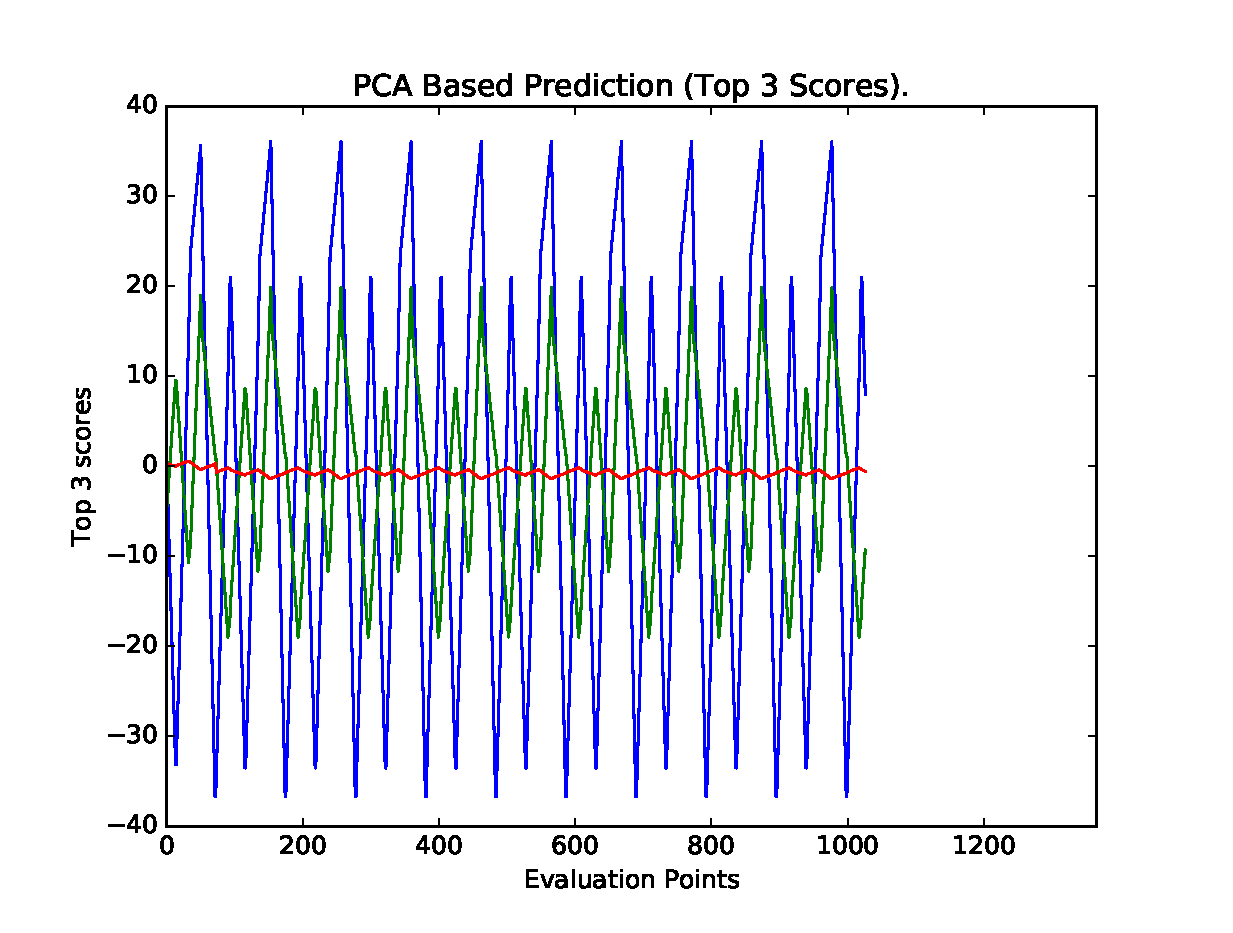
\includegraphics[width=0.85\textwidth]{Normal_Functioning_PCA.eps}
    \caption{\label{fig:NFP}Normal Functioning of Plant (PCA Top 3 scores (Blue, Green, Red))}
  \end{figure}
\end{frame}

\begin{frame}
  \begin{figure}
    \centering
    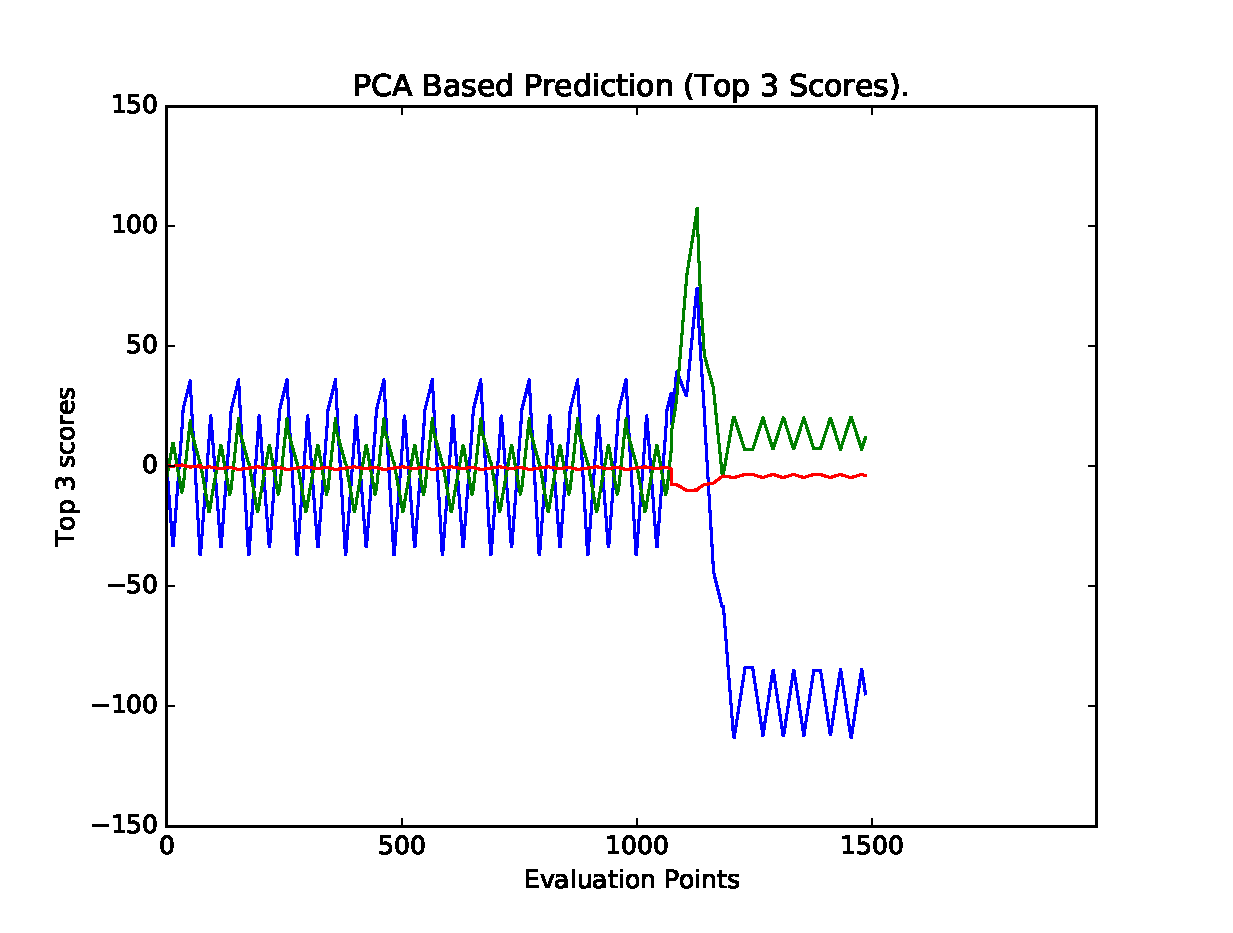
\includegraphics[width=0.85\textwidth]{Compromised_Functioning_PCA.eps}
    \caption{\label{fig:frog}PCA Top 3 Scores, plant compromised around evaluation point 1000}
  \end{figure}
  Notice how humorously the values in blue change. 
  
  Any on-site observer can notice it and shutdown the system.
\end{frame}

\section{Install a Brain in the Plant.}
\begin{frame}{Revisiting the Problem}
	What makes \textit{an attack}, \textbf{an attack}? 
\end{frame}
\begin{frame}{Anomaly!}
	Any anomalous behavior is bad for us. 
    
    Anything bad $\Rightarrow$ Shutdown the system
    
    Can we \textit{LEARN} what the normal working is?
\end{frame}
\begin{frame}{Neural Networks}
	Neural networks are extremely good at learning things, after-all they are modeled after neurons!
    
    They can \textit{learn} anything from recognizing objects to repetitive patterns.
    
    We'll be using a specific kind of an architecture, which currently excels at memorizing behaviors. 
\end{frame}
\begin{frame}{Long Short Term Memory (LSTM)\cite{hochreiter1997long}}
  \begin{figure}
    \centering
    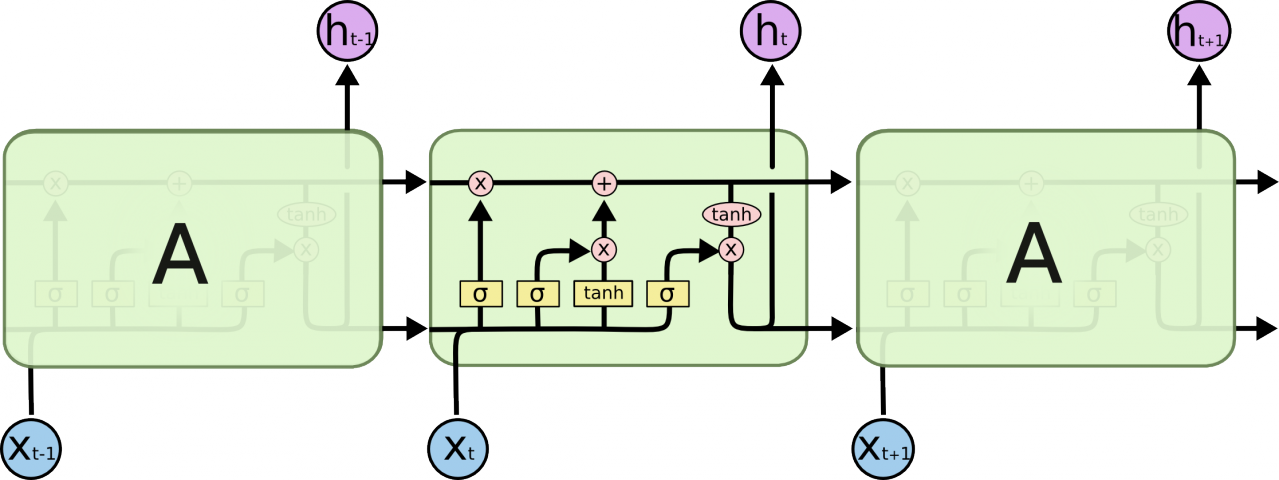
\includegraphics[width=0.85\textwidth]{lstm.png}
    \caption{\label{fig:lstm}Long Short Term Memory (LSTM) Units in action. Img: \href{http://colah.github.io/posts/2015-08-Understanding-LSTMs/}{colah}}
  \end{figure}
  LSTM is form of Recurrent Neural Network, it remembers what's important and forgets the trivial things.
  
  LSTM is capable of learning patterns in data and rejecting those that don't match. 
  
  Anomaly rejection! 
\end{frame}

\begin{frame}{LSTM Training}
	Before we use the brains, we need to teach them how our system works.
    
    We log the data (Process Variables) for sufficiently long period of normal working and \textit{train} the LSTM block accordingly.
    
    The output of the LSTM block is a confidence score evaluating to how close the current pattern is to regular working conditions.
\end{frame}

\begin{frame}
  \begin{figure}
    \centering
    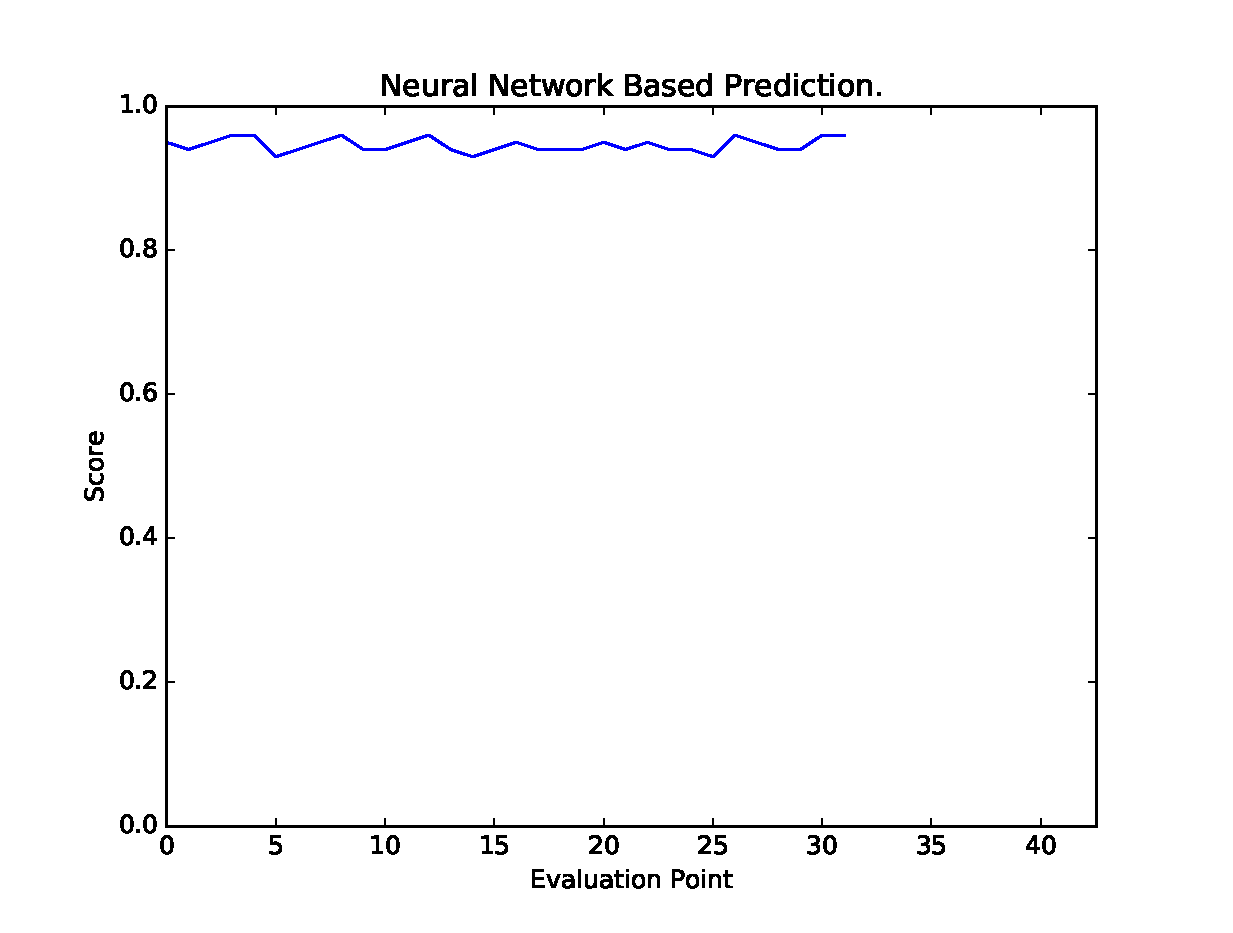
\includegraphics[width=0.85\textwidth]{Normal_Functioning_NN.eps}
    \caption{\label{fig:NFN}Normal Functioning of Plant (LSTM Confidence)}
  \end{figure}
  Notice the high levels of confidence (\textasciitilde 1)
\end{frame}

\begin{frame}
  \begin{figure}
    \centering
    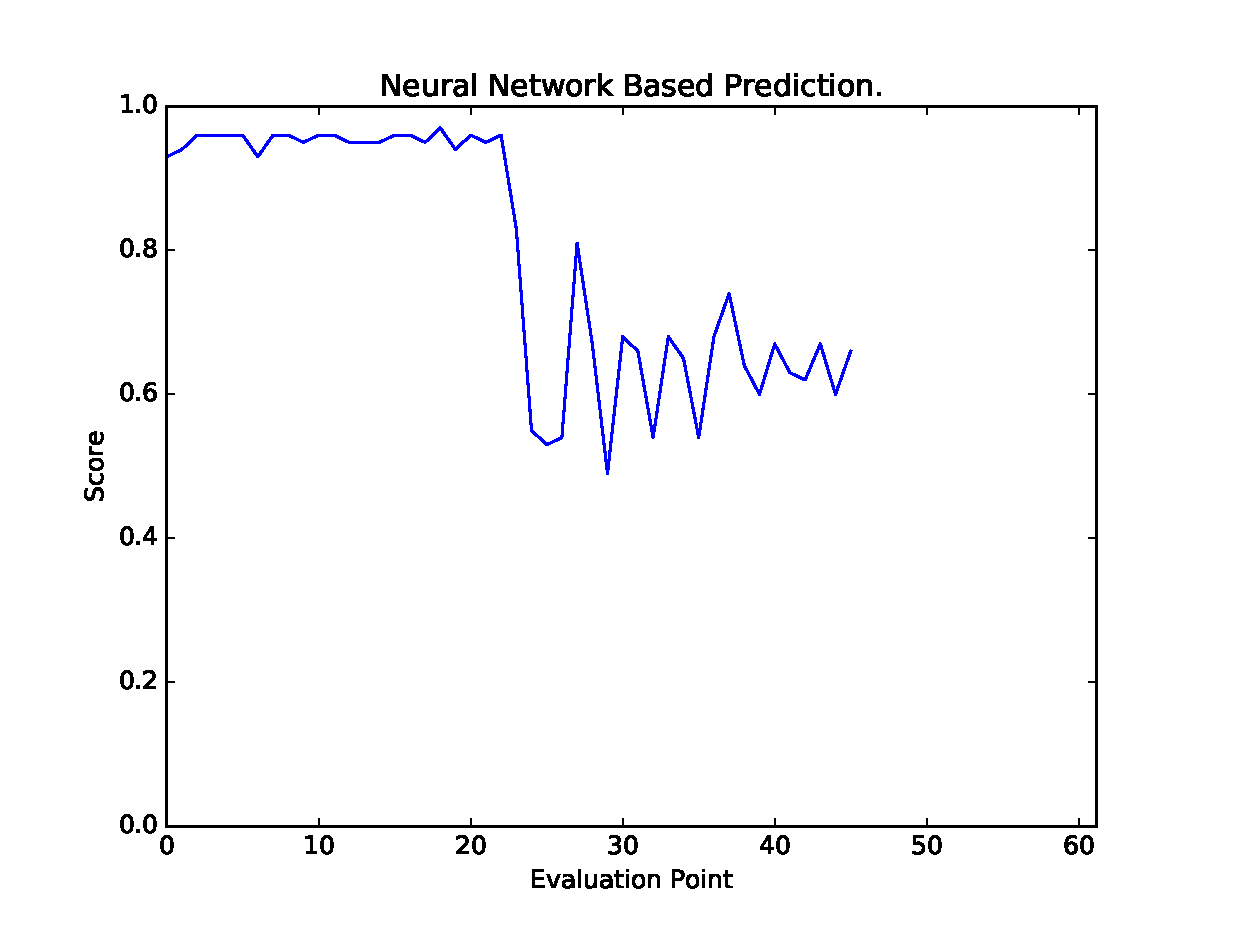
\includegraphics[width=0.85\textwidth]{Compromised_Functioning_NN.eps}
    \caption{\label{fig:CFN}LSTM Confidence Scores, plant compromised around evaluation point 20}
  \end{figure}
  Notice how significantly the confidence drops (\textasciitilde 40\% reduction!)
\end{frame}

\begin{frame}{Automation}
	LSTM based prediction paves way for an automated protocol in the event of an attack. (Difficult with PCA based method)
    
    As the regular working confidence is close to 1 any confidence value less than, say 0.8, might be considered as an attack.
    
    Further cases could be split on what action should be taken based on the confidence.
\end{frame}

\section{Summary}

\begin{frame}{Summary}
	We discussed how security aspects are handled in ICS.
    
    Zone division helps in minimizing damage, but yet needs to piggy back on a detection system.
    
    PCA based method is great in monitoring highly variable values when attacked.
    
    LSTM can learn to detect any anomaly and empower us with an automated damage control system.
  
\end{frame}

\begin{frame}{References}

  \bibliography{bib}
  \bibliographystyle{abbrv}
  \github \href{https://github.com/manikantareddyd/ics-attack-detection}{  Code Repository for the project}
\end{frame}



\begin{frame}{ }
	\begin{center}
		\LARGE{Thank You}
	\end{center}
    \begin{figure}
    	\centering
    	
\includegraphics[width=0.3\textwidth]{potato.eps}
    \end{figure}
   
\end{frame}

\end{document}
